\documentclass[a4paper,11pt]{report}
\usepackage[french]{babel}
\usepackage[T1]{fontenc}
\usepackage[utf8]{inputenc}
\usepackage{lmodern}
\usepackage{microtype}
\usepackage{hyperref}
\usepackage{tabulary}
\usepackage{framed}
\usepackage{fancyhdr}
\usepackage{amsmath}
\usepackage{bbm}
\usepackage{graphicx}
\usepackage{version}

\newcommand{\latin}[1]{\textit{#1}}

\usepackage{anysize}
%left,right, top, bottom
\marginsize{0.8in}{0.8in}{0.8in}{0.8in}


\pagestyle{empty}

\pagestyle{fancy}
\fancyhead{}
\renewcommand{\headrulewidth}{0.5pt}
\fancyhead[L]{\textit{\nouppercase{\leftmark}}}
\fancyfoot{}
\renewcommand{\footrulewidth}{0.5pt}
\fancyfoot[R]{\thepage}

\begin{document}
	\begin{titlepage}
		\vspace*{\stretch{2}}
		\begin{center}
			\large\bfseries\itshape Projet SF\\
		\end{center}
		\noindent\rule{\linewidth}{3pt}

		\begin{center}
			\Huge\bfseries\itshape RAPPORT\\
		\end{center}
		
		\noindent\rule{\linewidth}{3pt}
		\begin{center}
			\bfseries
			\large Modèlisation et Vérification du comportement de véhicules automatiques sur un pont à voie unique
			
		\end{center}
		\vspace*{\stretch{2}}
		\begin{center}
			Réalisé par \bfseries \itshape DOAN Cao Sang
		\end{center}
		\begin{center}
			\today
		\end{center}
	\end{titlepage}

\chapter{Propriété}
	{\huge \itshape L}e programme doit satisfaire les propriétés suivantes:
		\begin{enumerate}
			\item Il n'y a pas de collision (i.e. deux véhicules circulants en sens inverse) sur le pont.
			\item Un véhicule qui arrive est certain de passer sur le pont à l'issue d'une durée bornée.
		\end{enumerate}
	
\chapter{Explication}
\section{Question 1.1}
\subsection{Vaa}
	\begin{description}
		\item[VerificationA] est une place sortie, qui lie le composant \textit{Vaa} avec le contrôlleur \textit{CTRLP}, lorsque un véhicule A veut traverser le pont, d'abord il communique avec le contrôlleur \textit{CTRLP} pour avoir son autorisation.
		\item[OKControlleurA] est une place entrée qui lie entre \textit{Vaa} et \textit{CTRLP}, lorsque le \textit{Vaa} peut traverser sur le pont, le \textit{CTRLP} met son jeton pour que \textit{Vaa} puisse passer.
		\item[OKPont] est une place entrée qui lie le \textit{P} avec le \textit{Vaa}, le \textit{P} marque cette place lors qu'il reçoit l'autorisation de contrôlleur \textit{CTRLP}.
		\item[AuRevoirControlleurA] est une place sortie, le \textit{Vaa} marque cette place dès qu'il sort du \textit{P}.
	\end{description}	
	
	\subsection{Vab}
	\begin{description}
		\item[VerificationB] est une place sortie, qui lie le composant \textit{Vab} avec le contrôlleur \textit{CTRLP}, lorsque un véhicule B veut traverser le pont, d'abord il communique avec le contrôlleur \textit{CTRLP} pour avoir son autorisation.
		\item[OKControlleurB] est une place entrée qui lie entre \textit{Vab} et \textit{CTRLP}, lorsque le \textit{Vab} peut traverser sur le pont, le \textit{CTRLP} met son jeton pour que \textit{Vab} puisse passer.
		\item[OKPont] est une place entrée qui lie le \textit{P} avec le \textit{Vab}, le \textit{P} marque cette place lors qu'il reçoit l'autorisation de contrôlleur \textit{CTRLP}.
		\item[AuRevoirControlleurB] est une place sortie, le \textit{Vab} marque cette place dès qu'il sort du \textit{P}.
	\end{description}	
	
	\subsection{Pont}
	\begin{description}
		\item[CapaciteControlleur] est une place sortie, qui lie le composant \textit{P} avec le contrôlleur \textit{CTRLP} pour lui signaler sa capacité restante.
		\item[OKPont] est une place sortie qui lie le \textit{P} avec les 2 composants \textit{Vaa} et \textit{Vab}, le \textit{P} marque cette place lorsque sa capacité reste suffisante.
	\end{description}	
	
	\subsection{CTRLP}
	\begin{description}
		\item[VerificationA] est une place entrée, qui lie le composant \textit{Vaa} avec le contrôlleur \textit{CTRLP}, lorsque un véhicule A veut traverser le pont, le \textit{CTRLP} doit d'abord, recevoir sa demande.
		\item[VerificationB] est une place entrée, qui lie le composant \textit{Vab} avec le contrôlleur \textit{CTRLP}, lorsque un véhicule B veut traverser le pont, le \textit{CTRLP} doit d'abord, recevoir sa demande.
		\item[OKControlleurA] est une place sortie qui lie entre \textit{Vaa} et \textit{CTRLP}, lorsque le \textit{Vaa} peut traverser sur le pont, le \textit{CTRLP} met son jeton pour que \textit{Vaa} puisse passer.
		\item[OKControlleurB] est une place sortie qui lie entre \textit{Vab} et \textit{CTRLP}, lorsque le \textit{Vab} peut traverser sur le pont, le \textit{CTRLP} met son jeton pour que \textit{Vab} puisse passer.
		\item[CapaciteControlleur] est une place entrée, qui lie le composant \textit{P} avec le contrôlleur \textit{CTRLP} pour savoir la capacité restante du \textit{P}.
		\item[AuRevoirControlleurA] est une place entrée, cette place est marqué par le \textit{Vaa}.
		\item[AuRevoirControlleurB] est une place entrée, cette place est marqué par le \textit{Vab}.
	\end{description}	
	
\section{Question 1.2}
	Cette composant contient 8 places, dont 4 ont pour le rôle d'interface, et 3 transitions.
	
	La place \textbf{VehiculeA} modélise le véhicule A  lors qu'il arrive devant le pont. S'il veut passer sur le pont, d'abord, il communique avec le contrôlleur par la transition \textit{demanderEntrerA}, cette transition met un jeton dans l'interface \textbf{VerificationA} qui lie avec le contrôlleur \textit{CTRLP} et passe à l'état \textbf{AttenteAutorisationA}. Lorsqu'il reçoit l'autorisation du contrôlleur \textit{CTRLP} via l'interface \textbf{OKControlleurA} et celle du pont \textit{P} via l'interface \textbf{OKPont}, il peut traverser le pont, en passant à l'état \textbf{DansPontA}. Ensuite, quand il sort, il marque la place d'interface \textbf{AuRevoirControlleurA} et aussi passe à l'état \textbf{FiniA} par la transition \textit{sortPontA}.
	
	La sécurité est garantie car, pour passer à l'état \textbf{AttenteAutorisationA} le véhicule doit communiquer avec le contrôlleur \textit{CTRLP}. Pour entrer, il doit avoir l'autorisation du contrôlleur \textit{CTRLP} et consommer le jeton dans la place d'interface \textbf{OKPont},  cette place modélise la consommation de la capacité du pont \textit{P}. Enfin, il signale sa sortie du pont au contrôlleur \textit{CTRLP} en mettant un jeton dans la place \textbf{AuRevoirControlleurA}.

	\begin{figure}[!htbp]
		\centering
		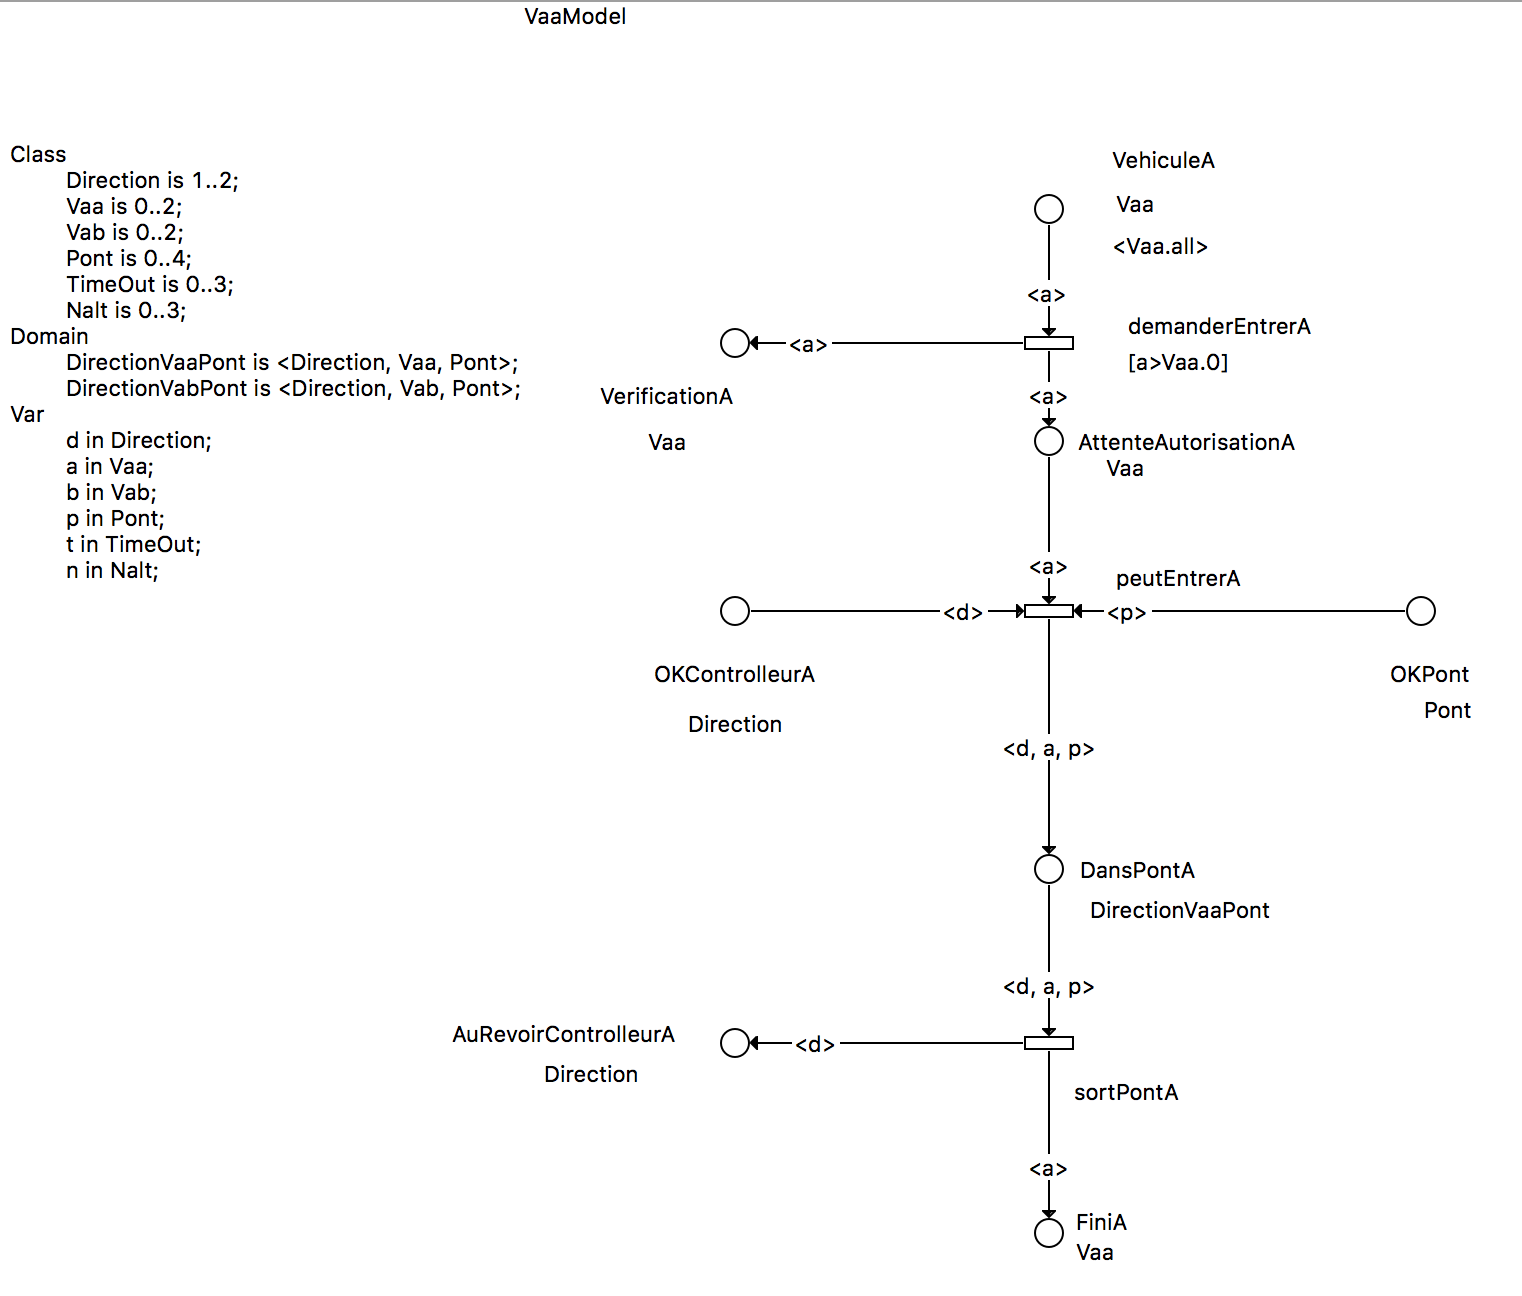
\includegraphics[width = 15cm]{vaaModel.png}
		\caption{Le composant modélise le véhicule automatisée A.}
	\end{figure}
	\newpage
	
\section{Question 1.3}
	Cette composant est identique avec celle de véhicule A, contient 8 places, dont 4 ont pour le rôle d'interface, et 3 transitions.
	
	La place \textbf{VehiculeB} modélise le véhicule B  lors qu'il arrive devant le pont. S'il veut passer sur le pont, d'abord, il communique avec le contrôlleur par la transition \textit{demanderEntrerB}, cette transition met un jeton dans l'interface \textbf{VerificationB} qui lie avec le contrôlleur \textit{CTRLP} et passe à l'état \textbf{AttenteAutorisationB}. Lorsqu'il reçoit l'autorisation du contrôlleur \textit{CTRLP} via l'interface \textbf{OKControlleurB} et celle du pont \textit{P} via l'interface \textbf{OKPont}, il peut traverser le pont, en passant à l'état \textbf{DansPontB}. Ensuite, quand il sort, il marque la place d'interface \textbf{AuRevoirControlleurB} et aussi passe à l'état \textbf{FiniB} par la transition \textit{sortPontB}.
	
	La sécurité est garantie car, pour passer à l'état \textbf{AttenteAutorisationB} le véhicule doit communiquer avec le contrôlleur \textit{CTRLP}. Pour entrer, il doit avoir l'autorisation du contrôlleur \textit{CTRLP} et consommer le jeton dans la place d'interface \textbf{OKPont},  cette place modélise la consommation de la capacité du pont \textit{P}. Enfin, il signale sa sortie du pont au contrôlleur \textit{CTRLP} en mettant un jeton dans la place \textbf{AuRevoirControlleurB}.

		\begin{figure}[!htbp]
		\centering
		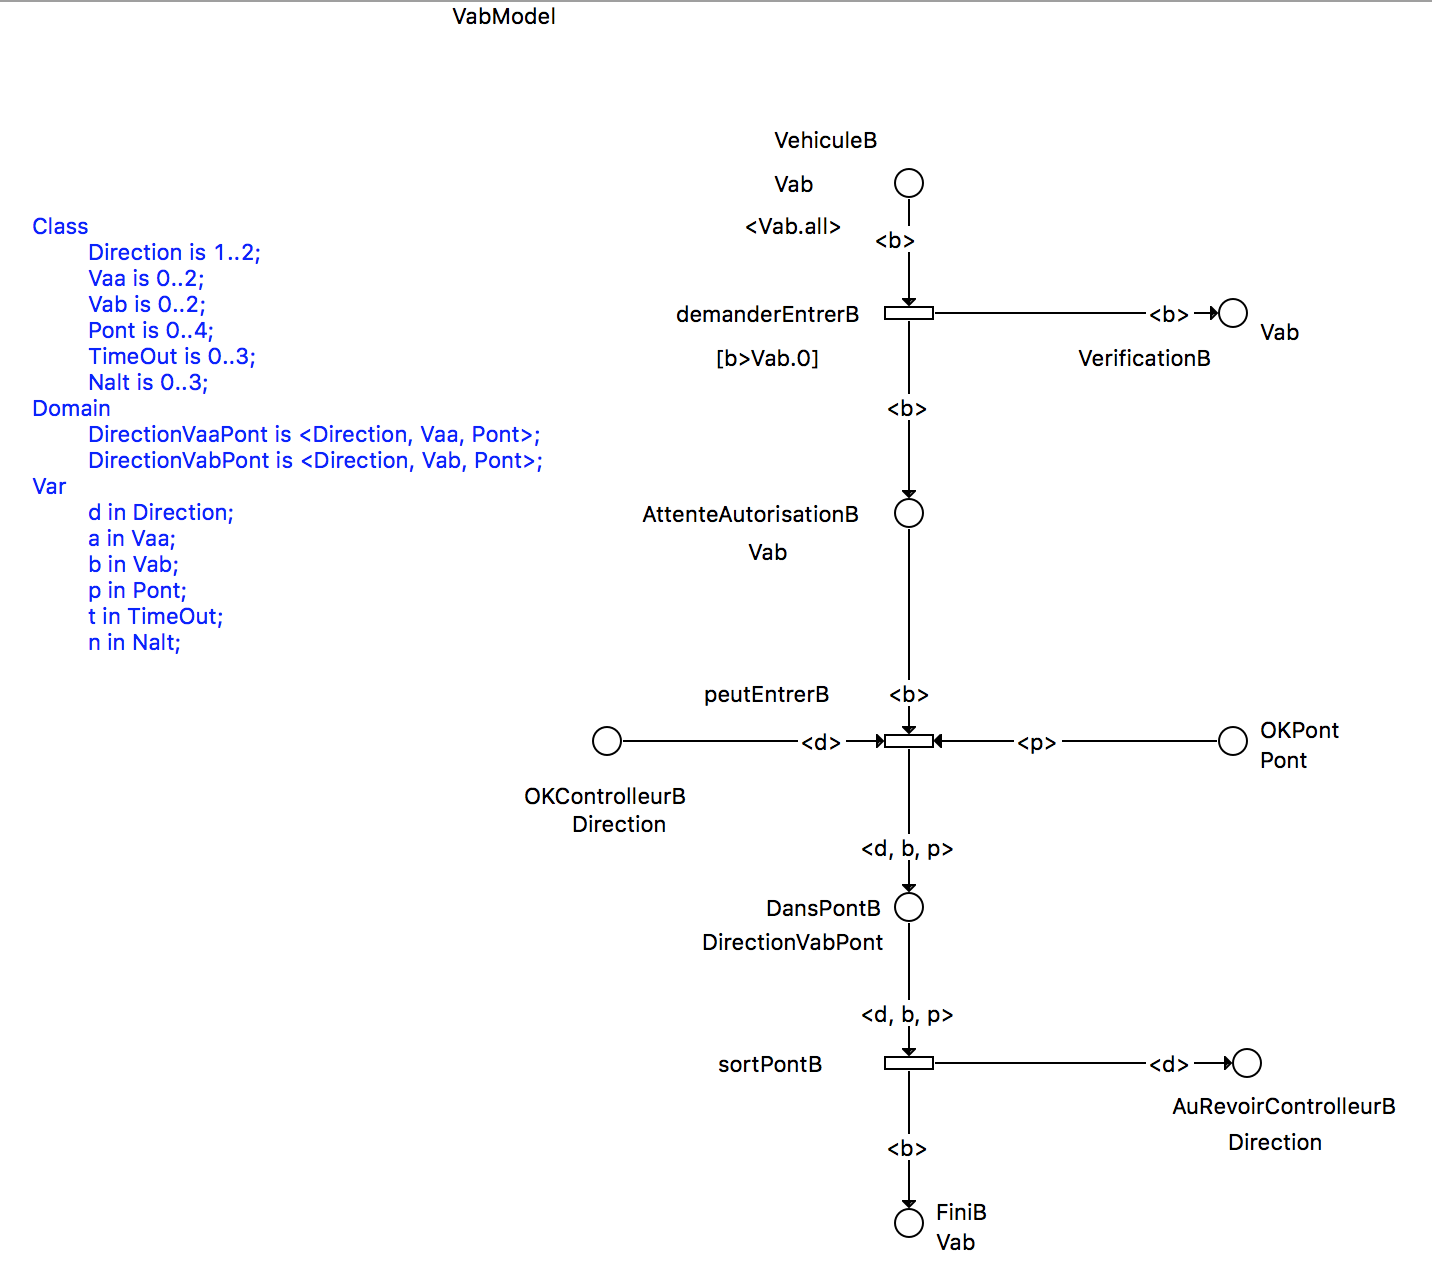
\includegraphics[width = 15cm]{vabModel.png}
		\caption{Le composant modélise le véhicule automatisée B.}
	\end{figure}
	\newpage
	
	
\section{Question 1.4}
	Le comportement d'un pont est simple, il notifie  sa capacité au contrôlleur \textit{CTRLP} et diminue si consomé par un véhicule. Donc, il contient 3 places, dont 2 interfaces et une transition.
	
	La transition \textit{notifieCapacite} marque 2 interfaces \textbf{CapaciteControlleur} et \textbf{OKPont} par 2 jetons, 1 pour chaque.

	\begin{figure}[!htbp]
		\centering
		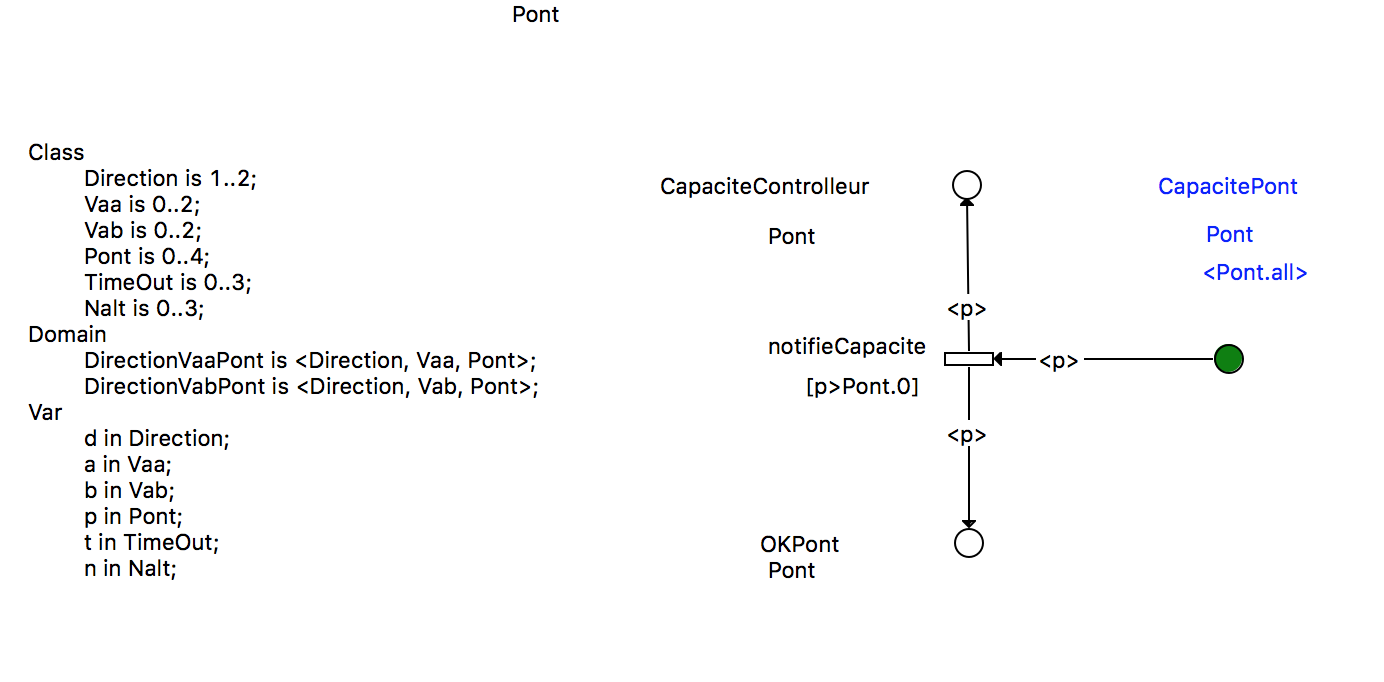
\includegraphics[width = 15cm]{pontModel.png}
		\caption{Le composant modélise le pont.}
	\end{figure}
	\newpage
	
\section{Question 1.5}
	Ce composant contient 12 places dont 7 interfaces, et 6 transitions.
	
	Lorsque le \textit{CTRLP} reçoit une demande d'entrer d'une véhicule \textit{Vaa} (idem, \textit{Vab}), il vérifie le sens actuel (initilise à 1, direction de A vers B) est correspondant à celui de \textit{Vaa}, le timeout restant, le nombre \textit{Nalt} restant et la capacité \textit{CapaP} restant du pont. Si ces conditions sont satisfaits, alors le contrôlleur \textit{CTRLP} donne l'autorisation au véhicule en attente. Quand le véhicule sort du pont, le contrôlleur reçoit son signal. 
	
	Le timeout est modélisé par une place nommée \textit{TimeOut} avec une seule transition \textit{ecoule}. Le \textit{TimeOut} décrémente une unité de temps automatique indépendamment avec le système. Lors de l'expiration de \textit{TimeOut}, il réinitialise le \textit{Nalt}, lui même, et change la direction actuelle.  Idem pour le \textit{Nalt}, si \textit{Nalt} = 0, il réinitialise le \textit{TimeOut}, \textit{Nalt} et change la direction.
	
	Quand la capacité du pont est à 0, alors aucun véhicule peut utiliser ce pont.

	\begin{figure}[!htbp]
		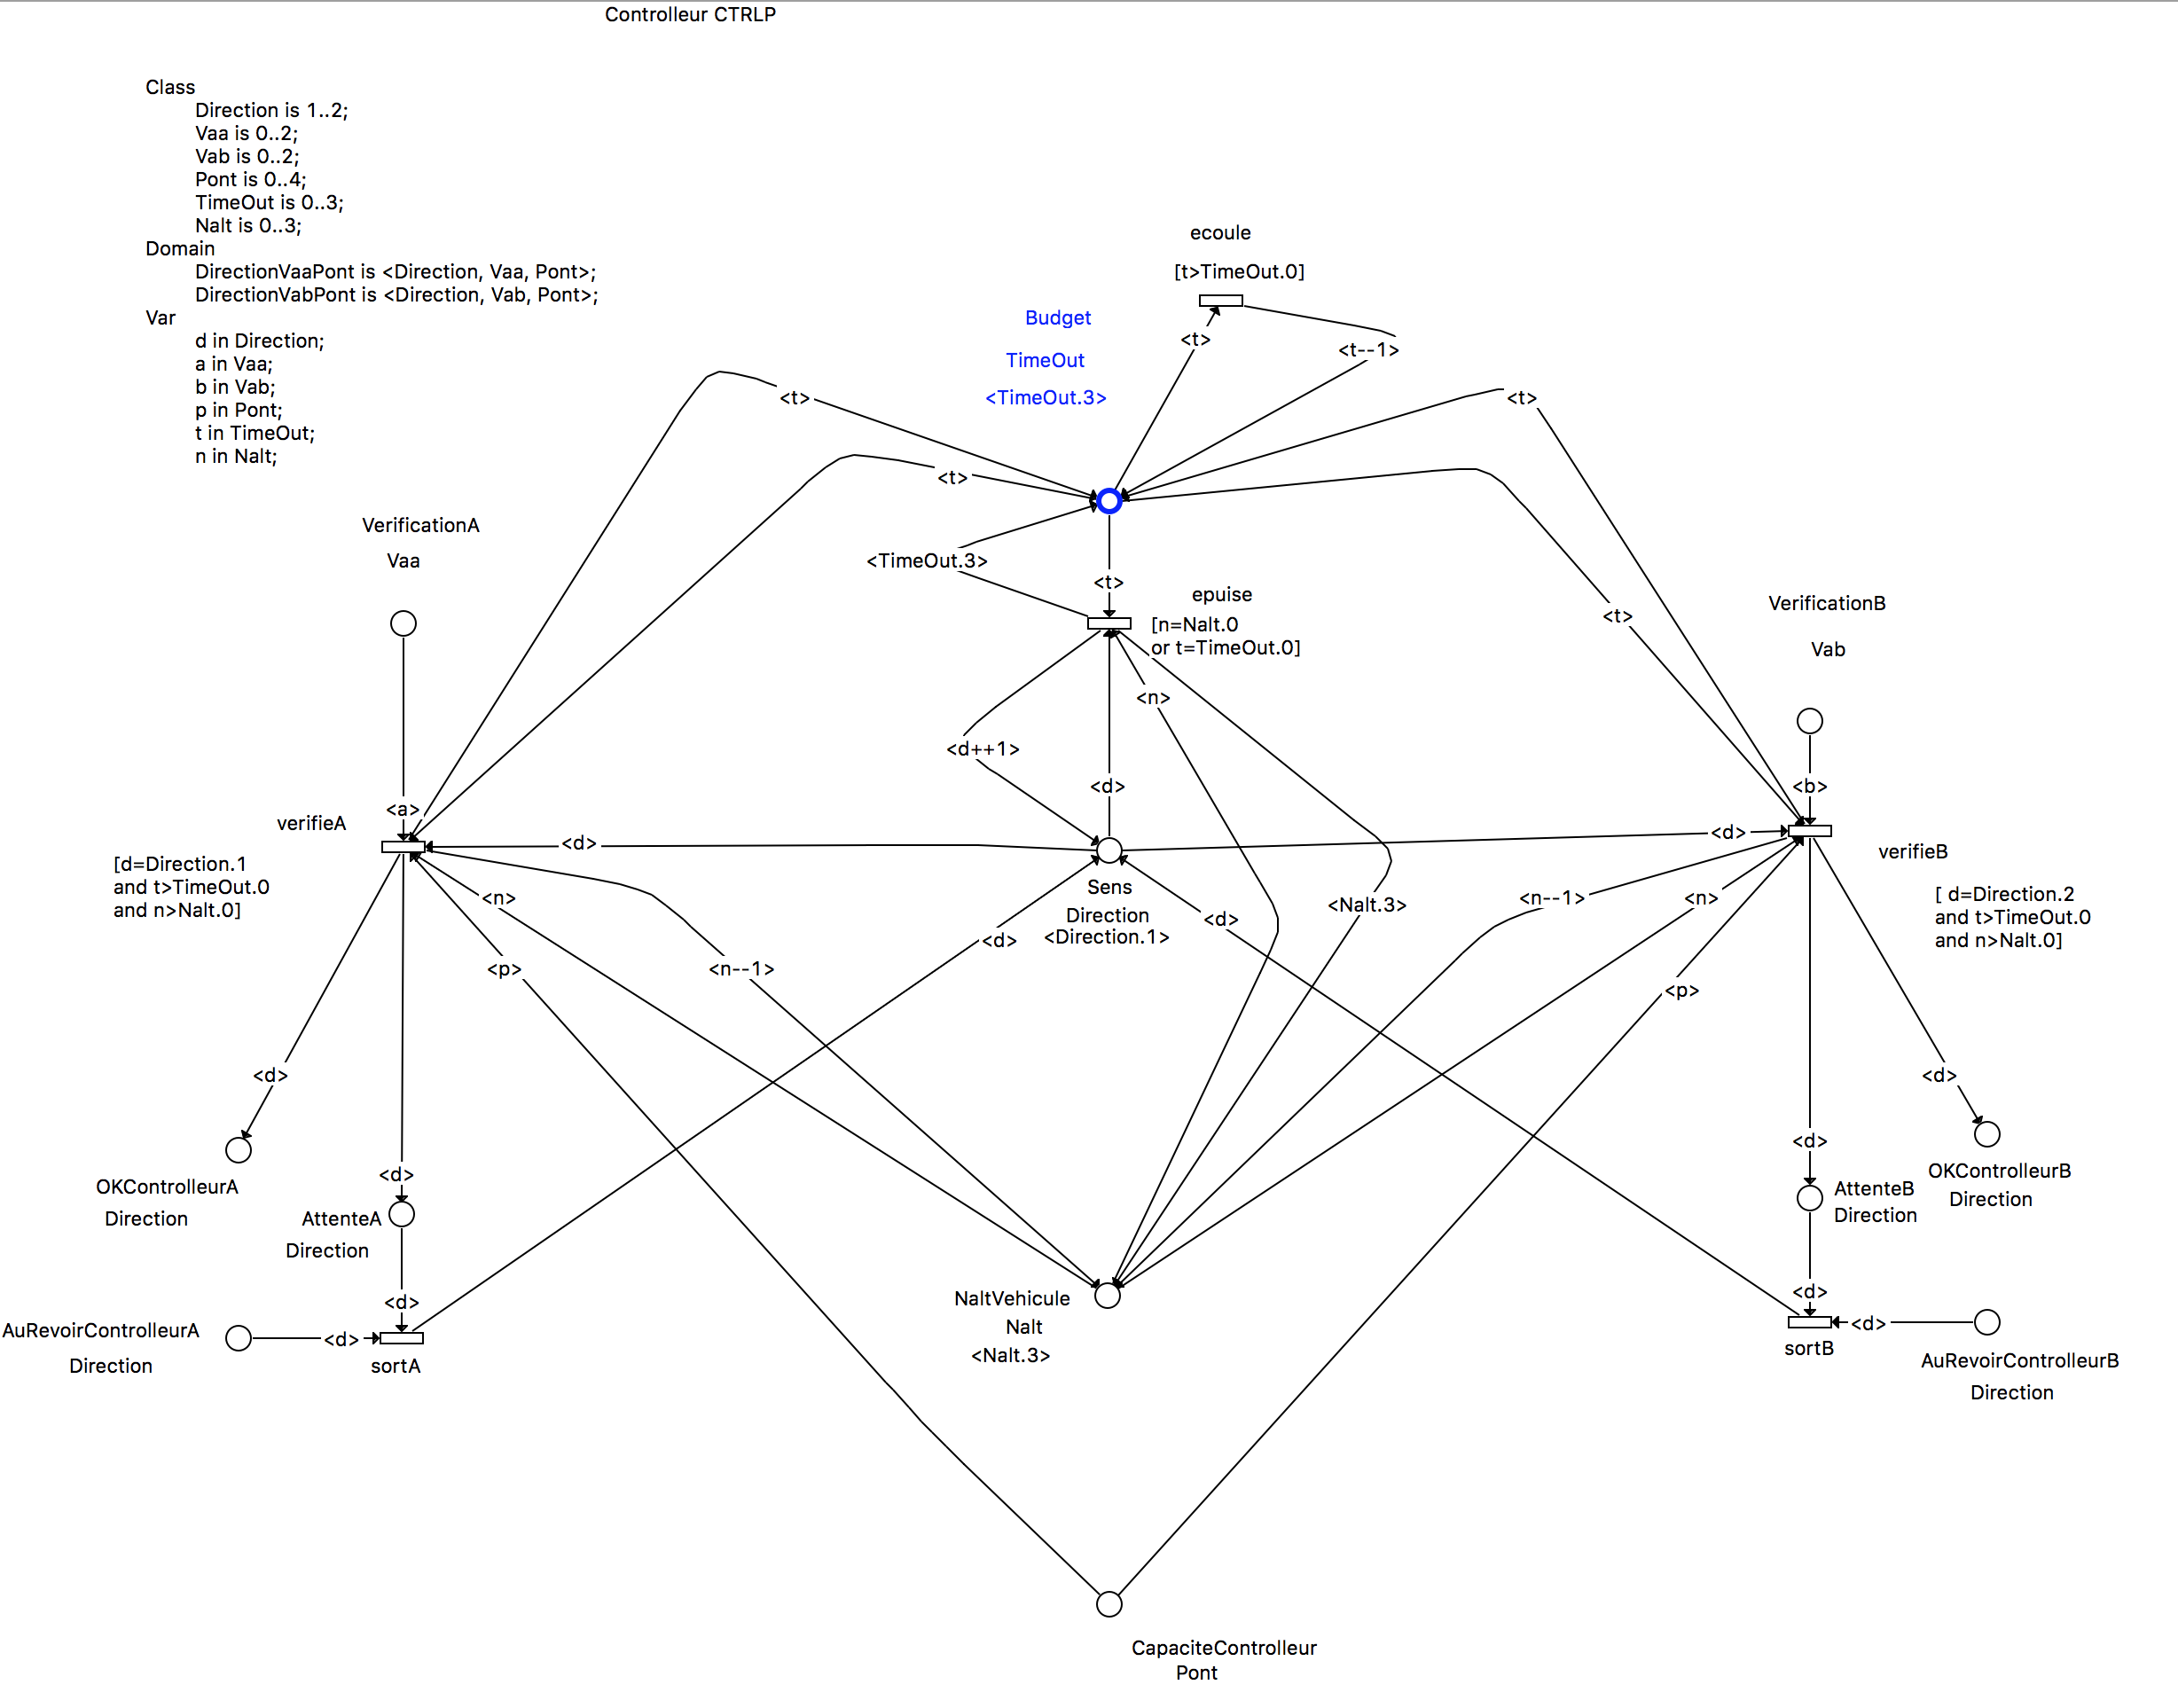
\includegraphics[width = 18cm]{ctrlpModel.png}
		\caption{Le composant modélise le pont.}
	\end{figure}
	\newpage
	
\section{Question 1.6}
	Cette assemblage contient 22 places, 13 transitions et 55$  $ arcs.
	
	\begin{figure}[!htbp]
		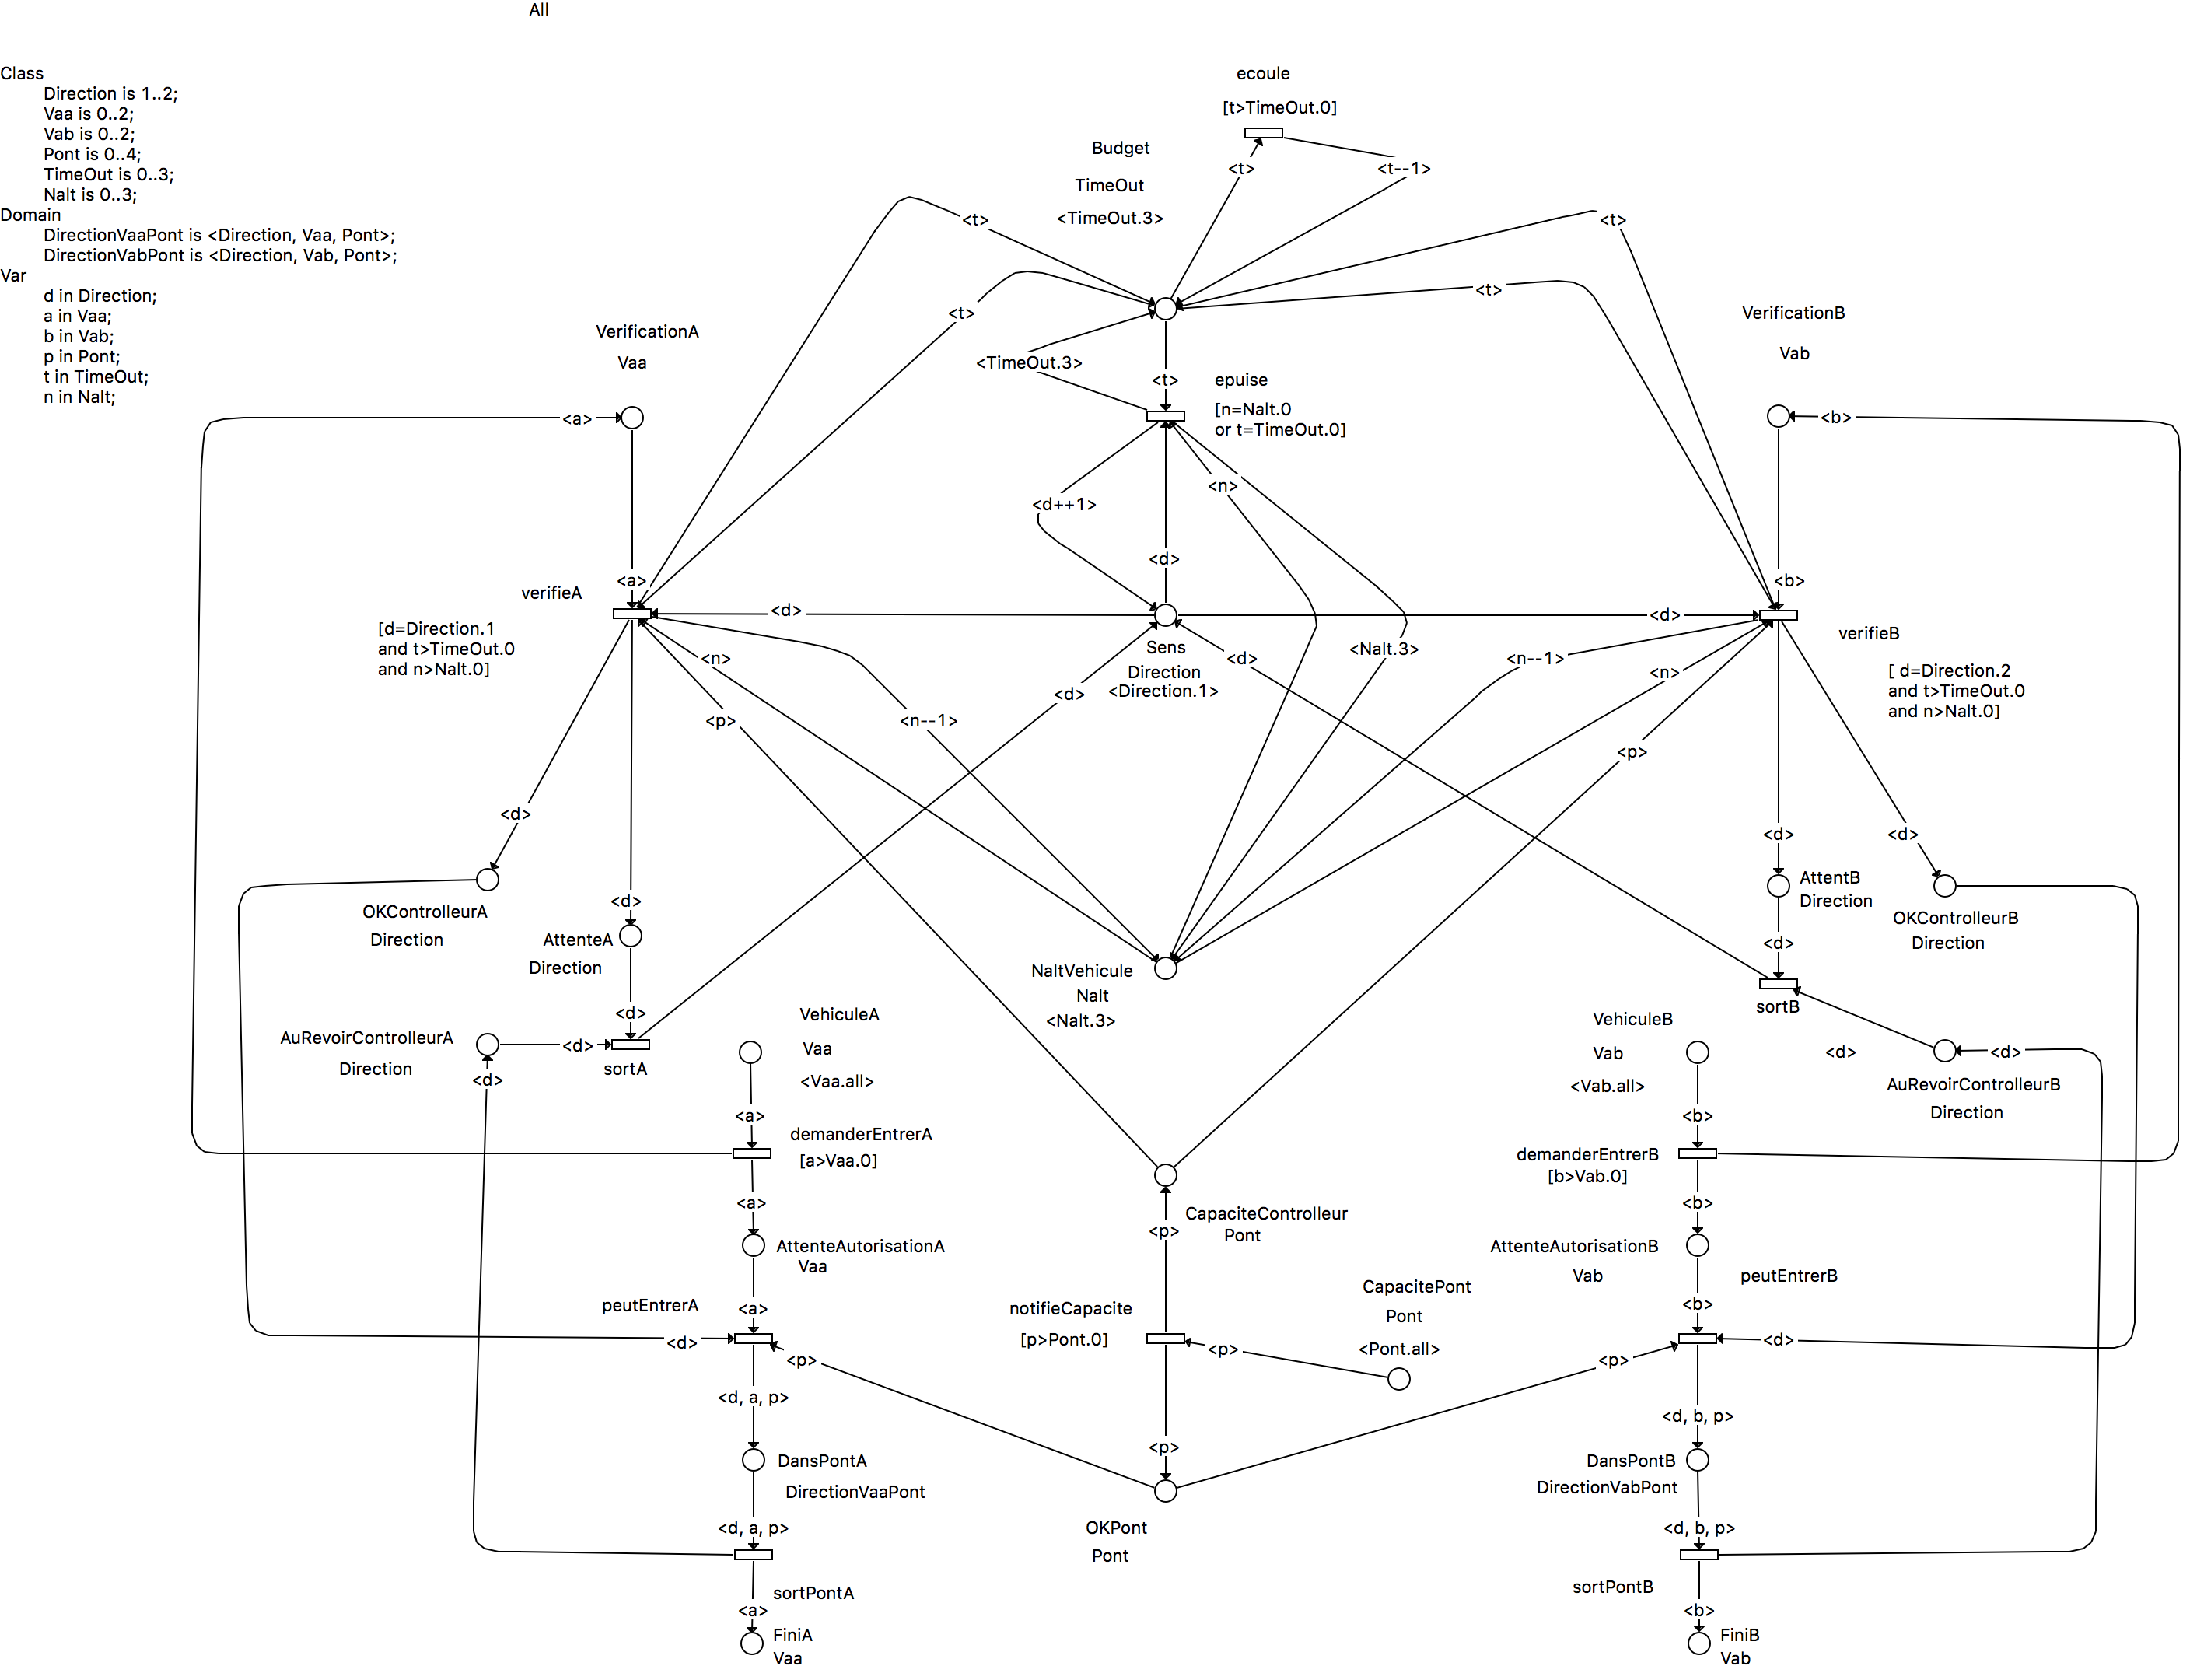
\includegraphics[width = 18cm]{allModel.png}
		\caption{Assemblage.}
	\end{figure}
	\newpage
	
\section{Question 1.7}
\subsubsection{Paramètres}
	Pour faciliter des vérifications car ma machine prend un temps énorme pour résoudre les formules. J'ai choisi:
	\begin{itemize}
		\item $N_{Vaa} = 2$
		\item $N_{Vab} = 2$
		\item $Capa_p = 4$
		\item $N_{Alt} = 3$
	\end{itemize}
	
	$Capa_p$ doit être supérieur au nombre total de véhicules, car sinon la propriété P2 ne peut être vérifiée.

\subsubsection{Vérification par CosyVerif4PN}
	Pour vérifier la propriété P1, \textit{"Il n'y a pas de collision (i.e. deux véhicules circulants en sens inverse) sur le pont."}, j'ai utilisé les formules suivantes:
	\begin{enumerate}
		\item \textit{query node ((card(DansPontA) + card(DansPontB)) == 2)} (Fichier P1\_1.txt)
		\item \textit{query node ((DansPontA == <.1.> and DansPontB == <.1.>) 
			\\or (DansPontA == <.1.> and DansPontB == <.2.>))} (Fichier P1\_2.txt)
		\item \textit{query node ((card(DansPontA)==1) and (card(DansPontB)==1))} (Fichier P1\_3.txt)
	\end{enumerate}
	
		Pour vérifier la propriété P2, \textit{"Un véhicule qui arrive est certain de passer sur le pont à l'issue d'une durée bornée."}, j'ai utilisé les formules suivantes:
		\begin{enumerate}
		\item 
			\textit{query verbose (AttenteAutorisationA==<.1.> and EG(DansPontA!=<.1.>))} (Fichier P2\_1.txt)
		\item
			\textit{query verbose (implies(AttenteAutorisationA==<.1.>, AF(DansPontA==<.1.>)) 
			\\and implies(AttenteAutorisationA==<.2.>, AF(DansPontA==<.2.>)) 
			\\and implies(AttenteAutorisationB==<.1.>, AF(DansPontB==<.1.>)) 
			\\and implies(AttenteAutorisationB==<.2.>, AF(DansPontB==<.2.>)))} (Fichier P2\_2.txt)
	\end{enumerate}
	
	Quelques formules pour les "autres propriétés triviales attendues":
		\begin{enumerate}
				\item \textit{query node ((card(VehiculeA) + card(AttenteAutorisationA) + card(DansPontA) + card(FiniA)) != 3)}. Le nombre de véhicules \textit{Vaa} reste constant. (Fichier P3\_1.txt)
				\item \textit{query node (card(CapacitePont) > 5)}. La capacité du pont $Capa_p$ est constante.(Fichier P3\_2.txt)
				\item \textit{query node (card(Budget) > 1)}. Il y a au plus 1 jeton dans la place \textbf{Budget} à la fois.(Fichier P3\_3.txt)
				\item \textit{query node (card(Sens) > 1)}. Il y a au plus 1 jeton dans la place \textbf{Sens} à la fois.(Fichier P3\_4.txt)
				\item \textit{query node (card(NaltVehicule) > 1)}. Il y a au plus 1 jeton dans la place \textbf{NaltVehicule} à la fois.(Fichier P3\_5.txt)
		\end{enumerate}

\section{Question 1.8}

	
\begin{comment}
\begin{verbatim}
query node ((card(DansPontA)==1) and (card(DansPontB)==1))

Number of places      22
Number of Queues      0
Number of Transitions 13
Number of arcs        55
Generating prod format
Generating and compiling code for the model
Generating the state space (this may take a while;-)

---
Statistics about the reachability graph provided by prod are shown below
Number of nodes: 283688
Number of arrows: 1033700
Number of terminal nodes: 0
Number of nodes that have been completely processed: 283688
Number of strongly connected components: 229305
Number of nontrivial terminal strongly connected components: 1
Evaluating the provided CTL formula
0 paths
Built set %1


query node (card(Sens) == 2) // oK 0 path

Statistics about the reachability graph provided by prod are shown below
Number of nodes: 283688
Number of arrows: 1033700
Number of terminal nodes: 0
Number of nodes that have been completely processed: 283688
Number of strongly connected components: 229305
Number of nontrivial terminal strongly connected components: 1
Evaluating the provided CTL formula
0 paths
Built set %1


query node ((DansPontA == <.1.> and DansPontB == <.1.>) or (DansPontA == <.1.> and DansPontB == <.2.>)) // OKKKK 0 path

Statistics about the reachability graph provided by prod are shown below
Number of nodes: 283688
Number of arrows: 1033700
Number of terminal nodes: 0
Number of nodes that have been completely processed: 283688
Number of strongly connected components: 229305
Number of nontrivial terminal strongly connected components: 1
Evaluating the provided CTL formula
0 paths
Built set %1

\end{verbatim}	
\end{comment}
\end{document}

